\subsubsection{February 2022}

Welcome to the February 2022 OpenSARLab Update!

\subparagraph{Changes:}

\begin{itemize}
\item Ubuntu 20.04.3 LTS
\item JupyterLab
\item Matplotlib widget
\item Url-widget
\item New memory monitor location
\item Notebook Debugger
\item Mamba
\item Mamba Gator
\item Spellchecker
\item Custom extensions
\item Recommended Jupyter Notebook changes related to update
\end{itemize}

\paragraph{Ubuntu 20.04.3 LTS}

\begin{itemize}
\item JupyterHub is now running on Ubuntu 20.04.3 LTS, updated from Ubuntu 18.04
\end{itemize}

\paragraph{JupyterLab}

\begin{itemize}
\item There are now JupyterLab profiles available alongside the Classic Jupyter Notebook profiles. JupyterLab comes with many more features than Classic Jupyter Notebook (see the \href{https://jupyterlab.readthedocs.io/en/stable/user/interface.html}{JupyterLab Docs}) for more information.
\item Classic Jupyter Notebook profiles will remain active for 1 month before being deprecated on March 7th.
\end{itemize}

\paragraph{Matplotlib widget}

\begin{itemize}
\item \texttt{matplotlib notebook} has been replaced with \texttt{matplotlib widget} for interactive matplotlib plots.\begin{itemize}
\item \texttt{matplotlib notebook} will not work in JupyterLab, whereas \texttt{matplotlib widget} works in both JupyterLab and Classic Jupyter Notebook.
\end{itemize}
\end{itemize}

\paragraph{Url-widget}

\begin{itemize}
\item The \texttt{url-widget} package is now installed, allowing notebook Python kernels access to the current notebook's URL.\begin{itemize}
\item This is useful for dynamically creating links to files and notebooks in OpenSARlab, and it is used in the kernel checking code at the beginning of ASF provided notebooks.
\end{itemize}
\end{itemize}

\paragraph{New Memory Monitor Location}

\begin{itemize}
\item JupyterLab comes with a built-in memory monitor, replacing the jupyter-resource-usage extension.\begin{itemize}
\item The new memory monitor can be found in the status bar at the bottom of the JupyterLab screen.
\end{itemize}
\end{itemize}

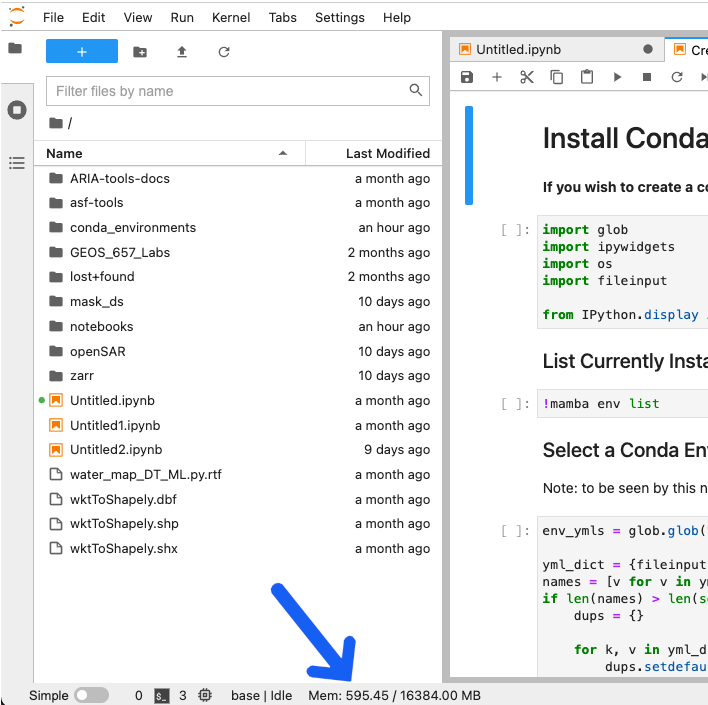
\includegraphics[width=0.7\linewidth]{files/memory_monitor-b336a1d9ea9c428bf307532d53b564ff.png}

\paragraph{Notebook Debugger}

\begin{itemize}
\item JupyterLab comes with a built-in notebook debugger.\begin{itemize}
\item \href{https://jupyterlab.readthedocs.io/en/stable/user/debugger.html}{JupyterLab Debugger Docs}
\end{itemize}
\end{itemize}

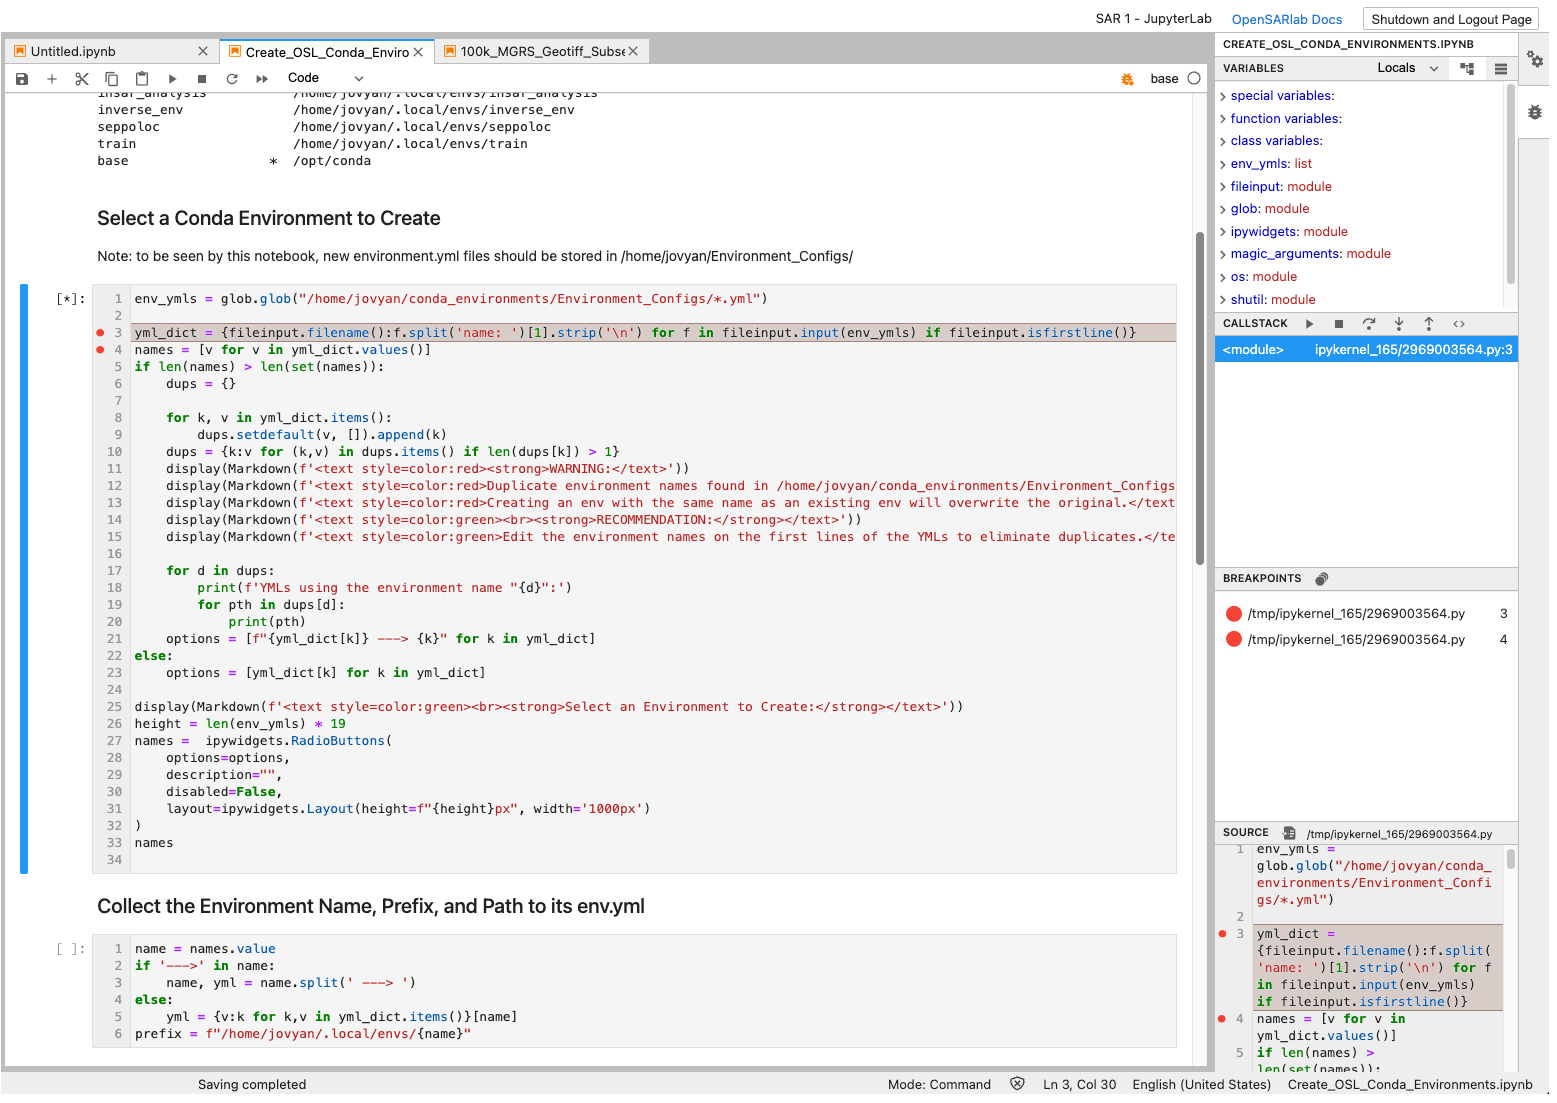
\includegraphics[width=0.7\linewidth]{files/debugger-c772ddfa3cdf2824afc44735f30281be.png}

\paragraph{Mamba}

\begin{itemize}
\item The \href{https://github.com/mamba-org/mamba}{mamba package manager} is now available in OpenSARlab.\begin{itemize}
\item Mamba is a multi-threaded ``reimplementation of the conda package manager in C++.''\begin{itemize}
\item It creates environments much more quickly than conda.
\end{itemize}
\end{itemize}


\item The \href{https://github.com/ASFOpenSARlab/opensarlab-envs}{opensarlab-envs repo} has been updated to use mamba.
\end{itemize}

\paragraph{Mamba Gator is installed}

\begin{itemize}
\item \href{https://github.com/mamba-org/gator}{mamba gator} provides a GUI for managing conda/mamba environments that is accessible in JupyterLab.\begin{itemize}
\item Access mamba gator by selecting the  \texttt{Conda Packages Manager} from the \texttt{Settings} menu.
\end{itemize}
\end{itemize}

\paragraph{Spellchecker}

\begin{itemize}
\item The \href{https://github.com/jupyterlab-contrib/spellchecker}{spellchecker extension} is installed.\begin{itemize}
\item It checks spelling in markdown cells.
\item The language may be changed in the status bar at the bottom of the screen.
\end{itemize}
\end{itemize}

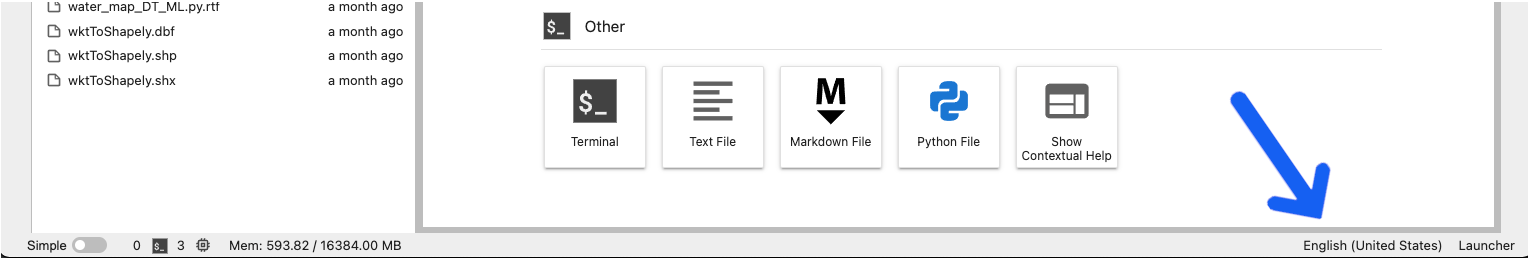
\includegraphics[width=0.7\linewidth]{files/language-7731ca45e6f15149a0b8842980445c71.png}

\paragraph{Custom Extensions}

\begin{itemize}
\item We have added some custom JupyterLab extensions to duplicate custom features previously added in OpenSARlab for Jupyter Notebooks.\begin{itemize}
\item \href{https://pypi.org/project/opensarlab-profile-label/}{opensarlab-profile-label} provides the name of the current OpenSARlab profile in the topbar.
\item \href{https://pypi.org/project/opensarlab-doc-link/}{opensarlab-doc-link} provides a link to the \href{https://opensarlab-docs.asf.alaska.edu/}{OpenSARlab documentation} in the topbar.
\item \href{https://pypi.org/project/opensarlab-controlbtn/}{opensarlab-controlbtn} provides a \texttt{Shutdown and Logout Page} button in the topbar.
\item \href{https://pypi.org/project/opensarlab-notifications/}{opensarlab-notifications} provides similar functionality to the popup notifications used in the OpenSARlab Classic Jupyter Notebook profiles.
\end{itemize}
\end{itemize}

\paragraph{Recommended Jupyter Notebook Changes}

The following bullet points cover code changes you may need to make to your notebooks for them to work in JupyterLab

\textit{note: These changes are backwards compatible and updated notebooks will still run in Jupyter Notebook.}

\textit{note: All \href{https://github.com/ASFOpenSARlab/opensarlab-notebooks}{ASF notebooks} have already been updated.}

\begin{itemize}
\item The javascript variable \texttt{Jupyter.notebook.kernel} does not exist in JupyterLab.\begin{itemize}
\item If you need a Python variable containing a notebook's current Python kernel, run:\begin{itemize}
\item \texttt{env = !echo \$CONDA\_PREFIX}
\end{itemize}
\end{itemize}


\item The javascript variable \texttt{window.location} does not exist in JupyterLab\begin{itemize}
\item If you need the current url of your Jupyter workspace, install the \texttt{url-widget} package in your conda environment and use it to retrieve the url:
\end{itemize}
\end{itemize}

\begin{verbatim}
# In one cell
import url_widget as url_w
notebook_url = url_w.URLWidget()
display(notebook_url)
\end{verbatim}

\begin{verbatim}
# In a following cell
notebook_url = notebook_url.value
\end{verbatim}

\begin{itemize}
\item \texttt{\%matplotlib notebook} does not work for interactive plotting in JupyterLab\begin{itemize}
\item Instead, use: \texttt{\%matplotlib widget}
\end{itemize}


\item \texttt{asf\_notebook.py} is deprecated and has been replaced with \texttt{opensarlab-lib}: \href{https://github.com/ASFOpenSARlab/opensarlab-lib}{https://github.com/ASFOpenSARlab/opensarlab-lib}\begin{itemize}
\item \texttt{asf\_notebook.py} still works (with deprecation warnings) but it is not being maintained.
\item Install \texttt{opensarlab-lib} with one of the following commands:\begin{itemize}
\item \texttt{python -m pip install opensarlab-lib}
\item \texttt{conda install -n \textless environment\_name\textgreater  -c conda-forge opensarlab-lib}
\end{itemize}


\item Alternatively, you may add \texttt{environment.yml} as a dependency and use it instead.
\end{itemize}
\end{itemize}